% --------------------------------------------------------------
% This is all preamble stuff that you don't have to worry about.
% Head down to where it says "Start here"
% --------------------------------------------------------------
 
\documentclass[12pt]{article}
 
\usepackage[margin=1in]{geometry} 
\usepackage{amsmath,amsthm,amssymb}
 
\newcommand{\N}{\mathbb{N}}
\newcommand{\Z}{\mathbb{Z}}
 
\newenvironment{theorem}[2][Theorem]{\begin{trivlist}
\item[\hskip \labelsep {\bfseries #1}\hskip \labelsep {\bfseries #2.}]}{\end{trivlist}}

\newenvironment{lemma}[2][Lemma]{\begin{trivlist}
\item[\hskip \labelsep {\bfseries #1}\hskip \labelsep {\bfseries #2.}]}{\end{trivlist}}

\newenvironment{exercise}[2][Exercise]{\begin{trivlist}
\item[\hskip \labelsep {\bfseries #1}\hskip \labelsep {\bfseries #2.}]}{\end{trivlist}}

\newenvironment{problem}[2][Problem]{\begin{trivlist}
\item[\hskip \labelsep {\bfseries #1}\hskip \labelsep {\bfseries #2}]}{\end{trivlist}}

\newenvironment{question}[2][Question]{\begin{trivlist}
\item[\hskip \labelsep {\bfseries #1}\hskip \labelsep {\bfseries #2.}]}{\end{trivlist}}

\newenvironment{corollary}[2][Corollary]{\begin{trivlist}
\item[\hskip \labelsep {\bfseries #1}\hskip \labelsep {\bfseries #2.}]}{\end{trivlist}}

\usepackage{graphicx}
\graphicspath{{./}}

\begin{document}
 
% --------------------------------------------------------------
%                         Start here
% --------------------------------------------------------------
 
\title{Homework 1}%replace X with the appropriate number
\author{Yunzhong He\\ %replace with your name
204010749} %if necessary, replace with your course title
 
\maketitle
 
\begin{problem}{1. Sequence of Coin Flips}
\item {a.} {\begin{math} P[X=k] = (1-p)^{k-1}p \end{math}}
\item {b.} {Proof:}
 	\begin{align*}
	  P[X \geq x_0] & = P[X\neq1, X\neq2, X\neq3, \dots, X\neq x_0-1]\\
			& = P[X\neq1] \cdot P[X\neq2 | X\neq1] \cdot P[X\neq3 | X\neq2] \dots P[X\neq x_0-2 | X\neq x_0-1]\\
			& = (1-p) \cdot \frac{(1-p)^2}{(1-p)^1} \dots \frac{(1-p)^{x_0-1}}{(1-p)^{x_0-2}} = (1-p)^{x_0-1}
 	\end{align*}
\item {c.}
	\begin{align*}
			P[p>1/2|x=1] & = \frac{P[X=1|p>1/2] \cdot P[p>1/2]}{P[X=1]}\\
			& = \frac{P[X=1|p>1/2] \cdot P[p>1/2]}{P[X=1|p>1/2] \cdot P[p>1/2] + P[X=1|p<=1/2] \cdot P[p<=1/2]}
			& = \frac{3}{4}
	\end{align*}
\end{problem}

\begin{problem} {2. Convex Functions and Information Theory}
\item {a.} {Proof:\\}
		$\forall x_1, x_2 \in \mathbb{R}$ and $t \in [0,1]$ we have
		$|tx_1+(1-t)x_2|\leq |tx_1| + |(1-t)x_2|$. Thus $f(x) = |x|$ is convex.
		$\forall x \in \mathbb{R}$ we have $\frac{de^x}{dx} = e^x > 0$, thus $f(x) = e^x$ is convex
		So $f(x) = |x| + e^x$  is convex
\item {b.}
		Since $H = \sum_i-log(Pr(\textbf{x}) \cdot Pr(\textbf{x}))$, where
		\begin{align*}
			& Pr(\textbf{x};p_1, p_2, \dots, p_k) = \frac{\Gamma(\Sigma_ix_i+1)}{\Pi_i\Gamma(x_i+1)}\Pi_{i=1}^kP_i^{x_i} \\
			& Let \ L(\textbf{x}, p_1, p_2, \dots, p_k, \lambda) = \sum_i^k-log(Pr(\textbf{x};p_1, p_2, \dots, p_k))Pr(\textbf{x};p_1, p_2, \dots, p_k) + \lambda(\sum_{i=1}^kx_i-1) 
		\end{align*}
		Solving $\nabla L = \textbf{0}$ we have $ p_1 = p_2 = p_3 = \dots p_k = 1/k$ which maximize the entropy.
\end{problem}

\begin{problem}{3. Linear Algebra}
\item {a.} {Proof:\\}
	Since X and EX ara real-valued vectors, $\Sigma = E[(X-EX)(X-EX)^T]$ is symmetric. \\
	For any u 
	\begin{align*}
	  \textbf{u}^T\Sigma \textbf{u} & = E[\textbf{u}^T(X-EX)(X-EX)^T\textbf{u}] \\
	    & = E[((X-EX)\textbf{u})^T((X-EX)\textbf{u})] \\
		& = ||((X-EX)\textbf{u}||^2 \geq 0
    \end{align*}
	Thus it is positive-semidefinite
\item {b.1} {C=A+B} eigenvectors: $u_1, u_2, u_3, \dots, u_D$ eigenvalues: $\alpha_1+\beta_1, \alpha_2+\beta_2, \dots, \alpha_D+\beta_D$
\item {b.2} {D=A-B} eigenvectors: $u_1, u_2, u_3, \dots, u_D$ eigenvalues: $\alpha_1-\beta_1, \alpha_2-\beta_2, \dots, \alpha_D+\beta_D$
\item {b.3} {E=AB} eigenvectors: $u_1, u_2, u_3, \dots, u_D$ eigenvalues: $\alpha_1\cdot\beta_1, \alpha_2\cdot\beta_2, \dots, \alpha_D\cdot\beta_D$
\item {b.4} {$E=A^{-1}B$} eigenvectors: $u_1, u_2, u_3, \dots, u_D$ eigenvalues: $\beta_1/\alpha_1, \beta_2/\alpha_2, \beta_3/\alpha_3, \dots, \beta_D/\alpha_D$
\end{problem}

\begin{problem}{4. KNN Classification}
\item{The code for this problem can be found in knn\_classify.m, knn\_classify\_single.m, one\_hot\_encoding.m and plot\_boundry.m. All of them are tested in octave 4.0, one\_hot\_encoding may not work very well on lower versions of octave}
\item{c.} Running KNN Classification on car\_train.data, with k = 1, 5, $\dots$, 23, we have obtained
different valid and train accuracy below. And we found that the highest validation accuracy happens at k=11, which is around 0.874.
\begin{table} [htb]
\centering
\begin{tabular} {|l|c|r|}
k   & valid\_accu & train\_accu\\
1   & 0.75578  & 0.77789\\
3   & 0.81234  & 0.83789\\
5   & 0.83290  & 0.88316\\
7   & 0.84062  & 0.89579\\
9   & 0.87661  & 0.89895\\
11  & 0.87404  & 0.89368\\
13  & 0.85604  & 0.88526\\
15  & 0.83290  & 0.87474\\
17  & 0.82776  & 0.86842\\
19  & 0.82519  & 0.86000\\
21  & 0.81491  & 0.85895\\
23  & 0.83033  & 0.85263\\
\end{tabular}
\end{table}
\item{d.} Running KNN Classification using boundry.m as training set, with k = 1,5,15,20, we plotted the following graphs.\\
		\begin{figure}[h!]
			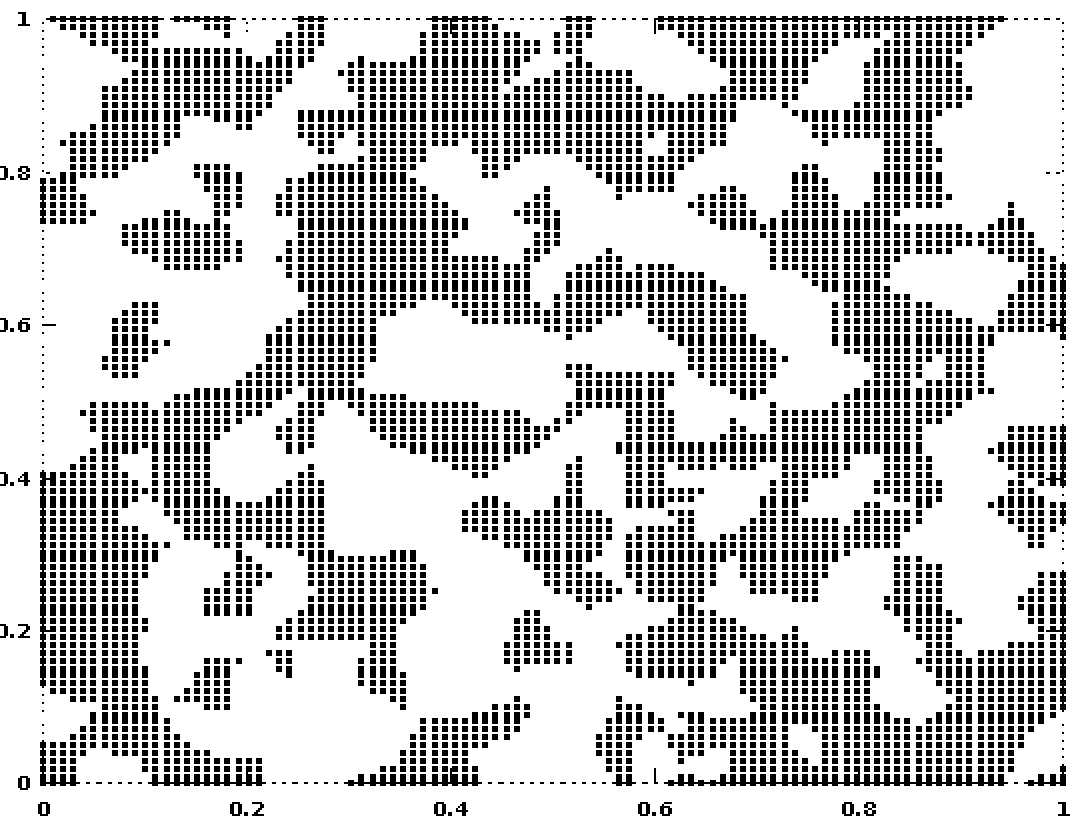
\includegraphics[height=5cm]{1.png}
			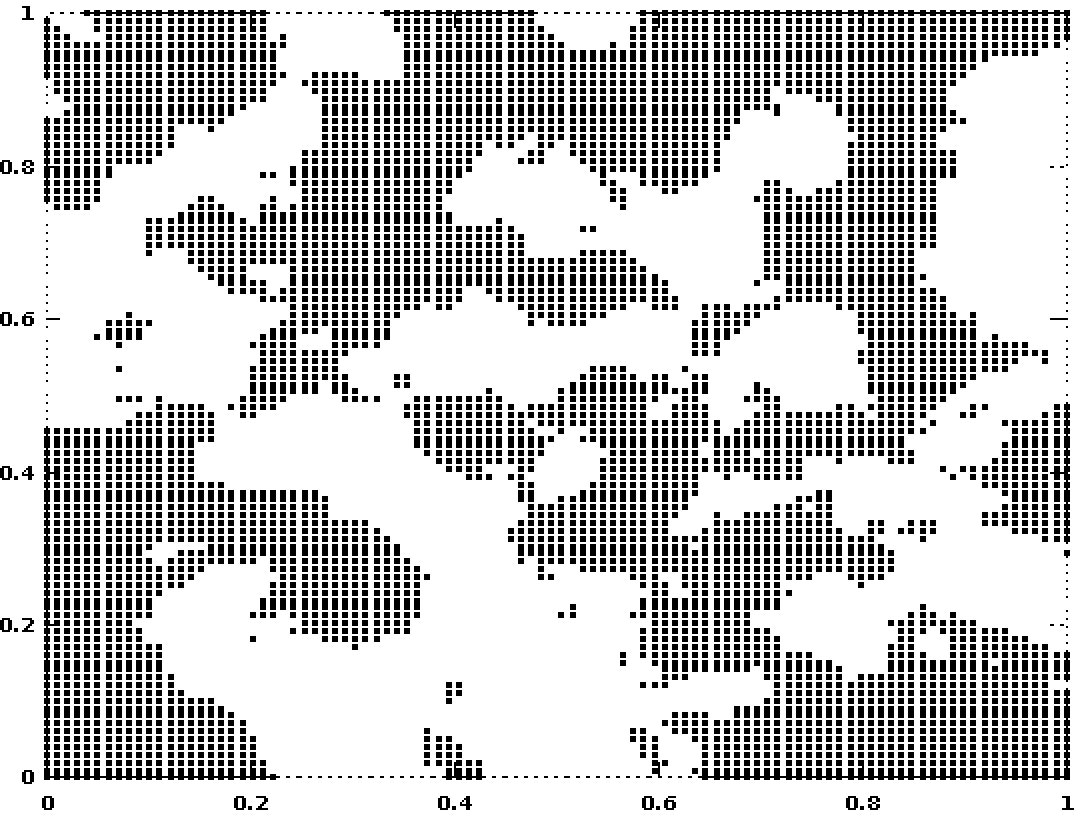
\includegraphics[height=5cm]{5.png}
			\caption{k=1(left), k=5(right)}
		\end{figure}\\	
		\begin{figure}[hb!]
			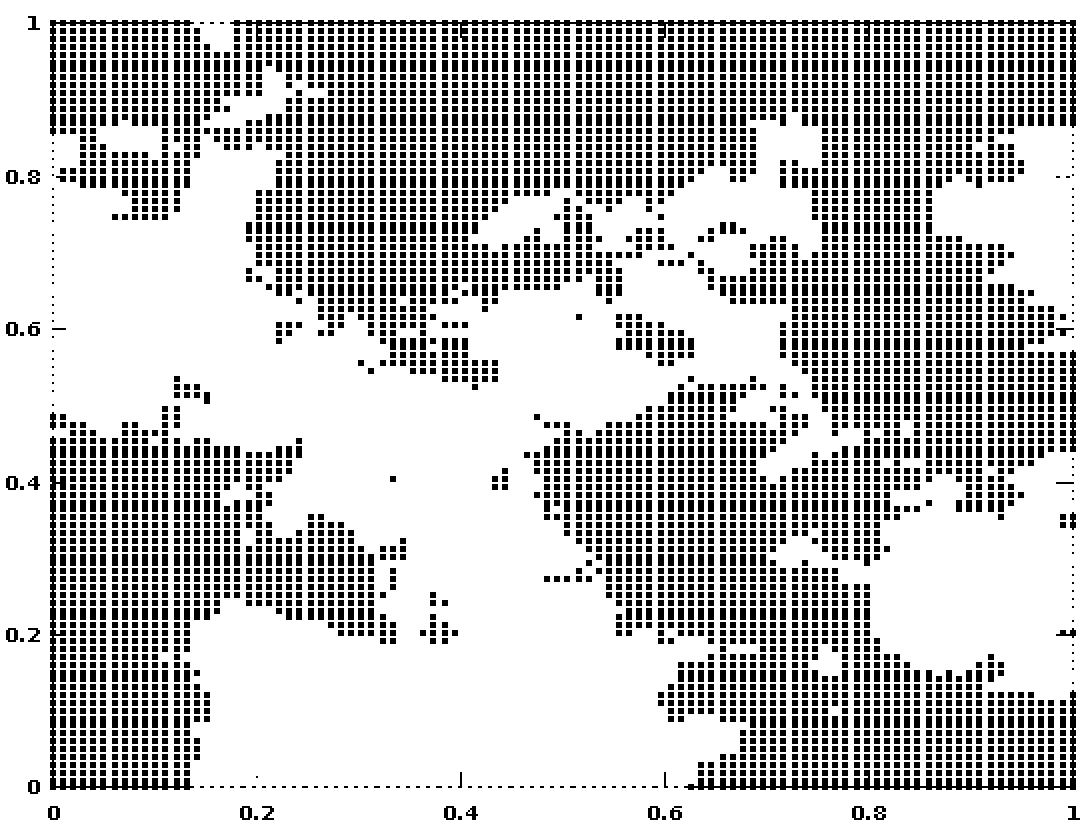
\includegraphics[height=5cm]{15.png}
			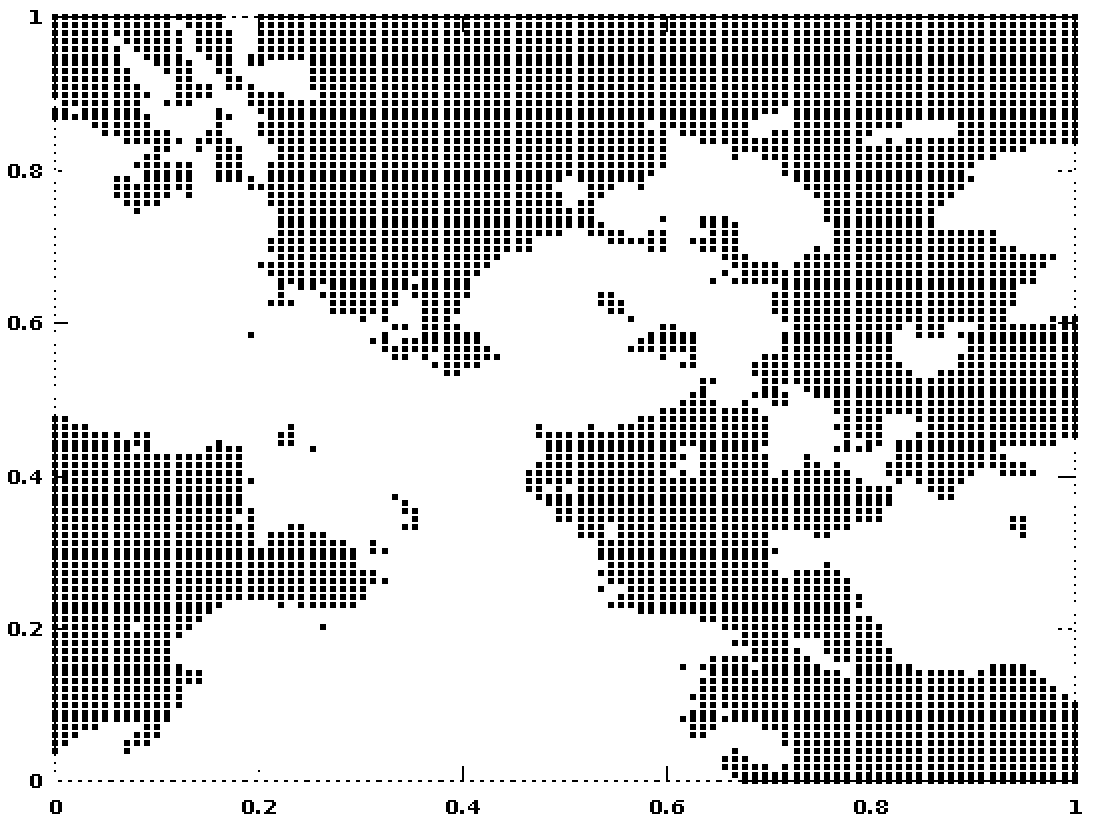
\includegraphics[height=5cm]{20.png}
			\caption{k=15(left), k=20(right)}
		\end{figure}\\
From Figure 1 and Figure 2 above we can see that the boundries are scattered when k=1 and k=5, and it gets significantly smoother when k=15 and k=20. So the smothness of the decision increases in this case.
\end{problem}

% --------------------------------------------------------------
%     You don't have to mess with anything below this line.
% --------------------------------------------------------------
 
\end{document}
